\documentclass[12pt, landscape]{article}
\usepackage[scaled=0.92]{helvet}
\usepackage{calc}
\usepackage{multicol}
\usepackage[a4paper,margin=3mm,landscape]{geometry}
\usepackage{amsmath,amsthm,amsfonts,amssymb}
\usepackage{color,graphicx,overpic}
\usepackage{hyperref}
\usepackage{newtxtext} 
\usepackage{enumitem}
\usepackage{esdiff}
\usepackage[table, dvipsnames]{xcolor}
\usepackage{mathtools}
\setlist{nosep}
\usepackage{tikz}
\usetikzlibrary{shapes.geometric}
\usepackage{makecell}  % for line break withih tabular

% for including images
\graphicspath{ {./images/} }

\pdfinfo{
  /Title (ma2104-midterm.pdf)
  /Creator (TeX)
  /Producer (pdfTeX 1.40.0)
  /Author (Yu Chenbo)
  /Subject (MA2104)
/Keywords (MA2104, nus, cheatsheet, pdf)}

% Turn off header and footer
\pagestyle{empty}

% redefine section commands to use less space
\makeatletter
\renewcommand{\section}{\@startsection{section}{1}{0mm}%
  {-1ex plus -.5ex minus -.2ex}%
  {0.5ex plus .2ex}%x
{\normalfont\large\bfseries}}
\renewcommand{\subsection}{\@startsection{subsection}{2}{0mm}%
  {-1explus -.5ex minus -.2ex}%
  {0.5ex plus .2ex}%
{\normalfont\normalsize\bfseries}}
\renewcommand{\subsubsection}{\@startsection{subsubsection}{3}{0mm}%
  {-1ex plus -.5ex minus -.2ex}%
  {1ex plus .2ex}%
{\normalfont\small\bfseries}}%
\makeatother

\renewcommand{\familydefault}{\sfdefault}
\renewcommand\rmdefault{\sfdefault}
%  makes nested numbering (e.g. 1.1.1, 1.1.2, etc)
\renewcommand{\labelenumii}{\theenumii}
\renewcommand{\theenumii}{\theenumi.\arabic{enumii}.}
\renewcommand\labelitemii{•}
\renewcommand\labelitemiii{•}

% \definecolor{mathblue}{cmyk}{1,.72,0,.38}
% \everymath\expandafter{\the\everymath \color{mathblue}}

% Don't print section numbers
\setcounter{secnumdepth}{0}

\setlength{\parindent}{0pt}
\setlength{\parskip}{0pt plus 0.5ex}
%% this changes all items (enumerate and itemize)
\setlength{\leftmargini}{0.5cm}
\setlength{\leftmarginii}{0.5cm}
\setlist[itemize,1]{leftmargin=2mm,labelindent=1mm,labelsep=1mm}
\setlist[itemize,2]{leftmargin=2mm,labelindent=1mm,labelsep=1mm}
\setlist[itemize,3]{leftmargin=2mm,labelindent=1mm,labelsep=1mm}

% adding my commands
% tightcenter
\newenvironment{tightcenter}{%
  \setlength\topsep{0pt}
  \setlength\parskip{0pt}
  \begin{center}
    }{%
  \end{center}
}

% boxed
\newenvironment{tightbox}{%
  \setlength\topsep{0pt}
  \setlength\parskip{0pt}
  \begin{center}
    \begin{tabular}{|@{\hspace{\dimexpr\fboxsep+0.5\arrayrulewidth}}c@{\hspace{\dimexpr\fboxsep+0.5\arrayrulewidth}}|}
      \hline
    }
    {%
    \\ \hline
    \end{tabular}
  \end{center}
}

% fixed width box
\newenvironment{fixedbox}[1][0.7]{
  \setlength\topsep{0pt}
  \setlength\parskip{0pt}
  \begin{center}
    \begin{tabular}{|>{\centering\arraybackslash}m{#1\linewidth}|}
    \hline
  }{
  \\ \hline
  \end{tabular}
  \end{center}
}

% definition of a new term
\usepackage{soul}
\definecolor{paleyellow}{RGB}{251,243,218}
\newcommand{\definition}[2][]{\sethlcolor{paleyellow}\hl{\textbf{#2}} #1  $\rightarrow$}
% inline definition
\newcommand{\ildefinition}[1]{\sethlcolor{paleyellow}\hl{\textbf{#1}}}

% important note (attention)
\newcommand{\attention}{{\color{red}\textbf{! }}}

% nice proof
\newenvironment{niceproof}[1][Proof]
{%
  \sbox0{\textit{#1}. }%
  \list{}{\labelwidth\wd0 \leftmargin\wd0 \labelsep 0pt }
\item[\usebox0]}
  {\endlist}


\usepackage{color, soul}
\usepackage{listings}
\usepackage{inconsolata}

\definecolor{codegreen}{rgb}{0,0.6,0}
\definecolor{codegray}{rgb}{0.5,0.5,0.5}
\definecolor{codepurple}{HTML}{C42043}
\definecolor{backcolour}{HTML}{F2F2F2}
\definecolor{bookColor}{cmyk}{0,0,0,0.90}

\newcommand{\code}[1]{\texttt{\sethlcolor{backcolour}\hl{$\,$#1$\,$}}}

% SQL code blocks
% define SQL styles
\lstdefinestyle{mySQL}{%
  language=SQL,
  backgroundcolor=\color{backcolour},
  commentstyle=\color{codegreen},
  keywordstyle=\color{codepurple},
  numberstyle=\numberstyle,
  stringstyle=\color{codepurple},
  basicstyle=\scriptsize\ttfamily,
  breaklines=true,
}

%  convenient absolute value symbol
\newcommand{\abs}[1]{\vert #1 \vert}

%  convenient floor and ceiling
\newcommand{\floor}[1]{\lfloor #1 \rfloor}
\newcommand{\ceil}[1]{\lceil #1 \rceil}

%  modulo with nicer spacing
\newcommand{\Mod}[1]{\ \mathrm{mod}\ #1}

%  convenient dx with nicer spacing
\newcommand{\dx}{\mathop{dx}}
\newcommand{\dy}{\mathop{dy}}


\usepackage{amssymb}

\DeclareRobustCommand{\ojoin}{\setbox0=\hbox{$\bowtie$}%
  \rule[-.02ex]{.25em}{.4pt}\llap{\rule[\ht0]{.25em}{.4pt}}}
\def\leftouterjoin{\mathbin{\ojoin\mkern-5.8mu\bowtie}}
\def\rightouterjoin{\mathbin{\bowtie\mkern-5.8mu\ojoin}}
\def\fullouterjoin{\mathbin{\ojoin\mkern-5.8mu\bowtie\mkern-5.8mu\ojoin}}

\newcommand\lojoin{\leftouterjoin}
\newcommand\rojoin{\rightouterjoin}
\newcommand\fojoin{\fullouterjoin}
\newcommand{\lsjoin}{\ltimes}

% aliasing commands
\newcommand{\ta}{\textbf{a}}
\newcommand{\tb}{\textbf{b}}
\newcommand{\tc}{\textbf{c}}
\newcommand{\tr}{\textbf{r}}
% -----------------------------------------------------------------------

\begin{document}
\raggedright
\begin{multicols*}{3}
  % multicol parameters
  % These lengths are set only within the two main columns
  \setlength{\columnseprule}{0.25pt}
  \setlength{\premulticols}{0.5pt}
  \setlength{\postmulticols}{1pt}
  \setlength{\multicolsep}{0.5pt}
  \setlength{\columnsep}{1pt}

  \begin{center}
    \fbox{%
      \parbox{0.8\linewidth}{\centering \textcolor{black}{
          {\Large\textbf{MA2104}}
        \\ \normalsize{AY24/25 SEM 1}}
        \\ {\textcolor{gray}{yyccbb}}
      }%
    }
  \end{center}

  \section{Vectors}
  \begin{itemize}
    \item $\ta\cdot\tb = \|\ta\|\|\tb\|\cos\theta$
    \item $\text{comp}_\ta \tb = \|\tb\|\cos\theta = \frac{\ta\cdot\tb}{\|\ta\|}$
    \item The vector projection: $\text{proj}_\ta \tb = \text{comp}_\ta \tb \times \frac{\ta}{\|\ta\|}$
    \item $\ta \times \tb = (a_2 b_3 - a_3 b_2)\textbf{i} - (a_1 b_3 - a_3 b_1)\textbf{j}
      + (a_1 b_2 - a_2 b_1)\textbf{k}$
    \item $\|\ta\times\tb\|=\|\ta\|\|\tb\|\sin\theta$
    \item $\ta\cdot(\tb\times\tc)=(\ta\times\tb)\cdot\tc=
      \begin{vmatrix}
        a_1 & a_2 & a_3 \\
        b_1 & b_2 & b_3 \\
        c_1 & c_2 & c_3
      \end{vmatrix}$ = volume of parallelepiped.
    \item Representations of a line: vector/parametric.
  \end{itemize}

  \subsection{Vector-valued Function}
  \begin{itemize}
    \item $\tr(t) = \langle f(t),g(t),h(t)\rangle$
    \item \tr(t) is a \underline{parametrization} of curve \textit{C}
    \item $\diff{}{t}(\tr(t)\times\textbf{s}(t)) = \tr'(t)\times\textbf{s}(t) + \tr(t)\times\textbf{s}'(t)$
    \item \textbf{Arc length}:
    \begin{itemize}
      \item Assumption: continuous, traversing \underline{exactly once}.
      \item $S = \int_{a}^{b}\sqrt{f'(t)^2+g'(t)^2+h'(t)^2}\,dt
        = \int_{a}^{b}\|\tr'(t)\|\,dt$
    \end{itemize}
  \end{itemize}

  \section{Cylinders and Quadric Surfaces}
  \begin{itemize}
    \item \definition[]{Cylinder} $\exists$plane P such that all the planes parallel to P interset the surface in the same curve.
    \item \begin{tabular}{|c|c|}
      \hline
      $\frac{x^2}{a^2} + \frac{y^2}{b^2} = \frac{z}{c}$ & elliptic paraboloid \\ \hline
      $\frac{x^2}{a^2} - \frac{y^2}{b^2} = \frac{z}{c}$ & hyperbolic paraboloid \\ \hline
      $\frac{x^2}{a^2} + \frac{y^2}{b^2} + \frac{z^2}{c^2} = 1$ & ellipsoid \\ \hline
      $\frac{x^2}{a^2} + \frac{y^2}{b^2} - \frac{z^2}{c^2} = 0$ & elliptic cone \\ \hline
      $\frac{x^2}{a^2} + \frac{y^2}{b^2} - \frac{z^2}{c^2} = 1$ & hyperboloid of one sheet \\ \hline
      $\frac{x^2}{a^2} + \frac{y^2}{b^2} - \frac{z^2}{c^2} = -1$ & hyperboloid of two sheets \\ \hline
    \end{tabular}
  \end{itemize}

  \section{Limits and Continuity}
  \begin{itemize}
    \item \definition[]{Continuous} f is continuous at (a,b) if $\lim_{(x,y)\to(a,b)}$ exists and is equal to f(a,b).
    \item A limit at (a,b) does not exist if the limits of f when approached from different paths do not agree.
    \item \textbf{How to prove a limit exists?} go polar!
    \begin{itemize}
      \item 2D: $x = r\cos\theta+a, y = r\sin\theta+b, r \rightarrow 0^+$ when approaching (a,b)
      \item 3D: $x=p\sin\phi\cos\theta,y=p\sin\phi\sin\theta,z=p\cos\phi,p\rightarrow 0^+$
      \item Squeeze Theorem:
      \item $\text{Since }\frac{x^4}{x^4+y^4}\leq 1\text{, }0\leq \left\lvert\frac{x^4 y}{x^4+y^4}\right\rvert = \left\lvert\frac{x^4}{x^4+y^4}y\right\rvert \leq |y|$
    \end{itemize}
  \end{itemize}

  \section{Partial Derivatives}
  \subsection{PDE Examples}
  \begin{itemize}
    \item Wave equation: $u_{tt}(x,t) = a^2u_{xx}(x,t)$
    \item Transport equation: $u_{t}(x,t) = u_{x}(x,t)$
    \item Heat diffusion: $u_{t}(x,t) = u_{xx}(x,t)$
    \item Laplace equation: $u_{xx}(x,y) + u_{yy}(x,y) = 0$
  \end{itemize}
  
  \subsection{Tangent Planes and Linear Approximations}
  \begin{itemize}
    \item Equation of tangent plane at (a,b): $z = f(a,b) + f_x(a,b)(x-a) + f_y(a,b)(y-b)$
    \item \textbf{Linearisation} of f at (a,b): L(x,y) = z
    \item f is \textbf{differentiable} at (a,b) if $f(x,y) \approx L(x,y)$
    \item Alternatively, f is differentiable if $f_x$ and $f_y$ exist near (a,b) and are continuous at (a,b).
    \item Total differential: $dz = f_x(x,y)dx + f_y(x,y)dy$
  \end{itemize}

  \subsection{The Chain Rule}
  \begin{itemize}
    \item $\diff{}{t}f(\tr(t)) = \nabla f(\tr(t))\cdot\tr'(t)$
    \item $\diffp{}{t}f(\tr(s,t)) = \nabla f(\tr(s,t))\cdot \diffp{}{t}\tr(s,t)$
  \end{itemize}

  \subsection{Implicit Differentiation}
  \begin{itemize}
    \item Idea: $G(x,y) = F(x(x,y),y(x,y),z(x,y))$, $G_x / G_y = 0$
    \item $\diffp{z}{x} = -\frac{F_x}{F_z}, \diffp{z}{y} = -\frac{F_y}{F_z}$
    \item Alternatively, apply $\diffp{}{x}$ and $\diffp{}{x} = \diffp{}{z}\diffp{z}{x}$.
  \end{itemize}

  \columnbreak

  \subsection{Directional Derivatives}
  \begin{itemize}
    \item $\nabla f(x_0,y_0)$ is normal to the level curve at $(x_0,y_0)$.
    \item For \textbf{unit vector} $\vec{u}$, $D_{\vec{u}}f(x,y) = \nabla f(x,y)\cdot\vec{u}$.
    \item $\vec{u}$, $D_{\vec{u}}f(x,y) = \nabla f\cdot\vec{u} = |\nabla f|\cos\theta$
  \end{itemize}

  \section{Extrema and Saddle Points, Lagrange Multipliers}
  \subsection{Extrema and Saddle Points}
  \begin{itemize}
    \item A point (a,b) is a \textbf{critical point} of f(x,y) if $\nabla f(a,b) = \vec{0}$ or if one of the partial derivatives does not exist.
    \item A \textbf{saddle point} is \textbf{NOT} a local extremum.
    \item (2nd Derivative Test)$D = \begin{vmatrix}
      f_{xx} & f_{xy} \\
      f_{yx} & f_{yy}
    \end{vmatrix} = f_{xx}f_{yy} - f_{xy}^2$
    \item $D<0$: saddle point.
    \item $D>0, f_{xx}>0$: minimum.
    \item $D>0, f_{xx}<0$: maximum.
    \item $D=0$: no information.
  \end{itemize}

  \subsection{Lagrange Multipliers}
  \begin{itemize}
    \item Scenario: optimise f(x,y) restricted to constraint g(x,y)=c
    \item $\nabla f \parallel \nabla g, \nabla f =\lambda\nabla g$
    \item System of equations: $\nabla f =\lambda\nabla g, g(x,y)=c$
    \item \textbf{Case of two constraints}
    \begin{itemize}
      \item Idea: optimise along a constraint curve in 4D
      \item 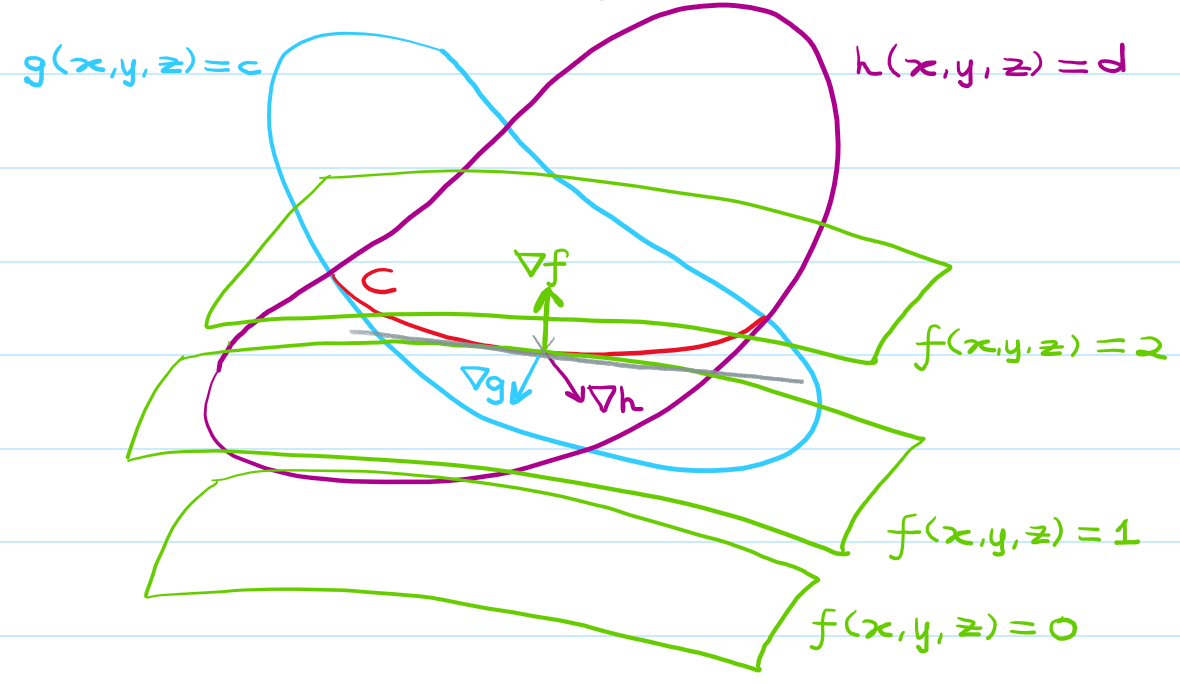
\includegraphics[width=\linewidth]{ma2104-midterm-2-lagrange.png}
      \item $\nabla f = \lambda\nabla g + \mu\nabla h$ (because $\nabla f, \nabla g, \nabla h$ are coplanar).
    \end{itemize}
  \end{itemize}
  

\end{multicols*}

\end{document}